\newpage
\section{SIMULACIONES DE SEGUIMIENTO DE CARGA} \label{simulaciones_seguimiento_de_carga}

\subsection{Seguimiento de carga} \label{seguimiento_de_carga}

Tradicionalmente, por razones técnicas y económicas, las centrales nucleares se han empleado para la generación de energía eléctrica como \textbf{centrales base}\footnote{Se denomina ``centrales base'' a aquellas plantas generadoras de elevada potencia cuya función es suministrar energía eléctrica de forma permanente, ofreciendo así un abastecimiento base fiable que cubra gran parte de la demanda eléctrica. Operan durante largos períodos contínuos, evitando en la medida de lo posible cualquier interrupción. Se incluye en este grupo a las centrales térmicas ---carbón, gas natural\dots---, nucleares e hidráulicas con gran capacidad de generación.}. Desde el punto de vista técnico, es complicado equilibrar las poblaciones neutrónicas del núcleo del reactor, mantener constante la eliminación de calor residual del núcleo y garantizar la integridad física de los compomenentes estructurales, cuando se dan variaciones de temperatura derivadas de las variaciones de potencia requeridas para el seguimiento de carga. Desde el punto de vista económico, debido a los elevados costes de capital inicial y a los reducidos costes de combustible, las centrales nucleares suministran electricidad al menor precio posible cuando mantienen un elevado \gls{factor de carga}, por lo que interesa que funcionen a plena potencia (\cite{stanford_load_following}).

Sin embargo, últimamente ha aumentado el interés en la capacidad de seguimiento de carga de las plantas nucleares, principalmente, en los siguientes dos casos concretos:

\begin{itemize}
  \item \textbf{Redes eléctricas donde la energía nuclear representa una gran parte de la generación energética total}, como es el caso de Francia (63 \%), Ontario (51 \%), Ucrania (56 \%), Carolina del Sur (55 \%), Illinois (52 \%)\dots En estos casos interesa que esta fuente de energía, al ser mayoritaria, tenga capacidad de adaptación a las habituales fluctuaciones de la demanda eléctrica diarias y a lo largo de las distintas épocas del año.
  \item \textbf{Redes eléctricas donde las fuentes de energía renovable intermitentes ---como la solar y la eólica--- constituyen una parte importante de la producción eléctrica total} y presentan importantes variaciones en la producción. Algunos casos en los que se da esta segunda situación son Alemania, España, Ontario, Nueva York, California\dots (\cite{ANS_2019}).
\end{itemize} 

\subsubsection{Tipos de maniobras de seguimiento de carga}

Por lo general, se definen tres tipos de maniobras de seguimiento de carga: 

\begin{itemize}
  \item \underline{Regulación primaria de frecuencia:} La demanda de electricidad nunca puede determinarse de antemano con precisión exacta, por lo que existe una cierta variación aleatoria en la demanda que resulta en fluctuaciones de frecuencia generalmente inferiores a 20 mHz. Las centrales nucleares deben monitorear la frecuencia en la red y adaptar inmediatamente su producción para mantener la frecuencia estable en el valor deseado. 
  
  El control de frecuencia primario permite ajustes a corto plazo en la producción de electricidad de acuerdo con la demanda cada 2 - 30 segundos.  En este caso, las correspondientes modulaciones de potencia suelen realizarse dentro de un rango del $\pm 2\%$ de la potencia nominal.
  \item \underline{Regulación secundaria de frecuencia:} Actúa en marcos de tiempo más largos ---desde varios segundos hasta varios minutos--- y restablece la frecuencia exacta calculando una desviación promedio de frecuencia durante un período de tiempo determinado. Con este fin, el operador de la red envía una señal a la central nuclear para modificar su nivel de potencia dentro de un rango del $\pm 5\%$ de la potencia nominal.
  
  \begin{figure}[h]
    \centering
    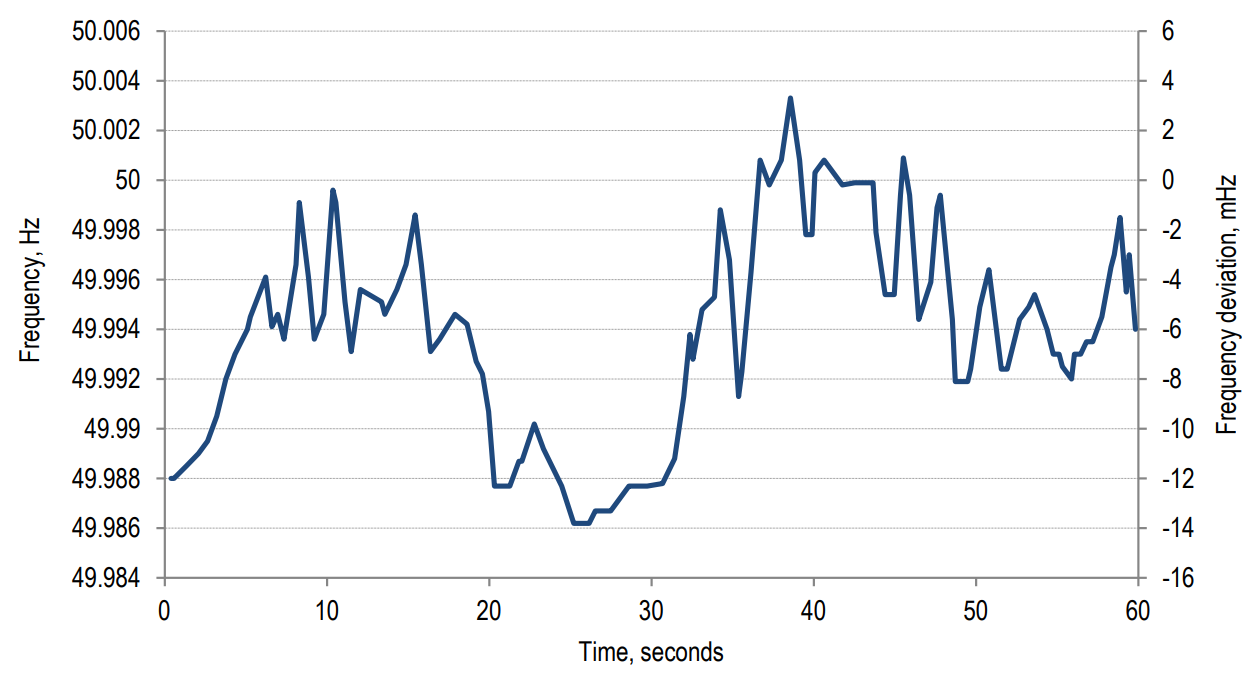
\includegraphics[width=0.7\textwidth]{content/figures/frequency_variation.png}
    \caption{Ejemplo de variaciones en la frecuencia de la red europea (\cite{NEA_2011_load_following}).}
    \label{fig:frequency_variations}
  \end{figure}

  \item \underline{Programas de carga variable predefinidos:} Reducciones o aumentos en la producción de energía acordados previamente con el operador de la red. Se suele tratar de una o dos variaciones de potencia al día, dependiendo de la demanda y de la capacidad de seguimiento de carga de la planta.
  
  \begin{figure}[h]
    \centering
    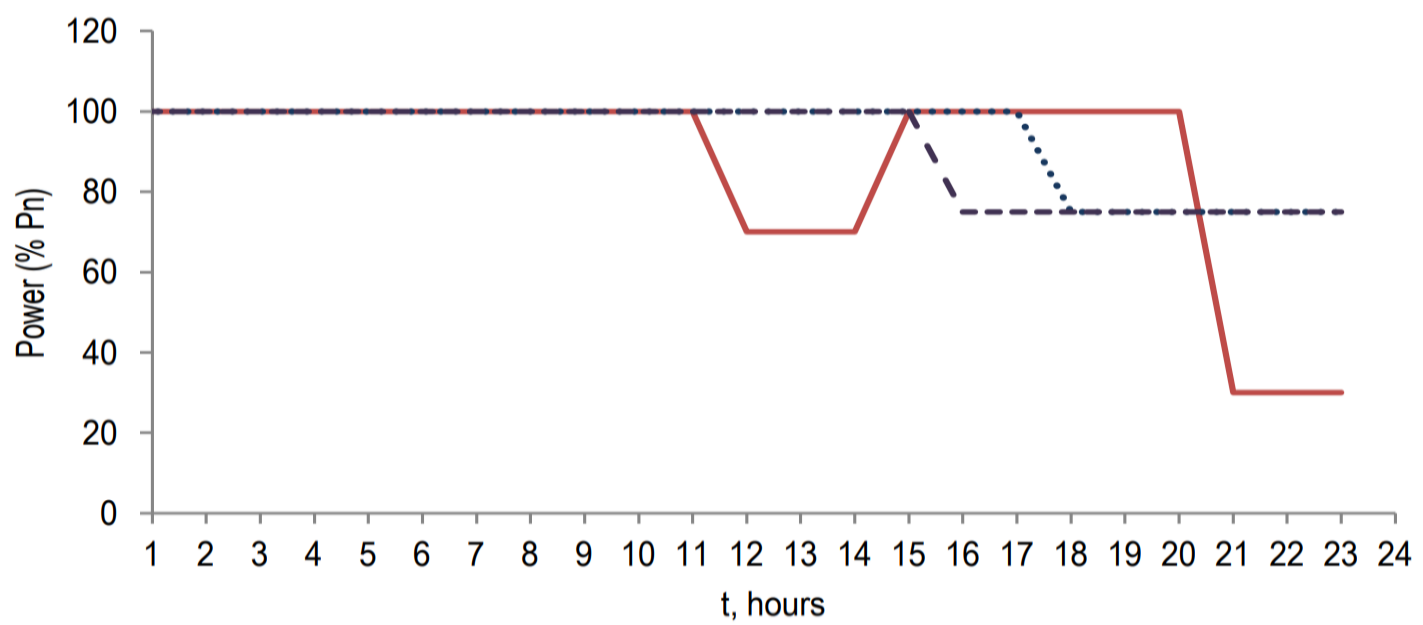
\includegraphics[width=0.7\textwidth]{content/figures/predefined_load_following.png}
    \caption{Ejemplo de un programa de carga variable predefinido para un período de 24 horas, en el que se producen dos reducciones importantes de potencia (\cite{NEA_2011_load_following}).}
    \label{fig:predefined_load_following}
    \vspace{-0.5cm}
  \end{figure}
\end{itemize}

\subsubsection{Capacidades de seguimiento de carga}

Vale la pena tener en cuenta los órdenes de magnitud que muestran cuantitativamente la capacidad de seguimiento de carga de la mayoría de centrales nucleares de gran escala. Estas, se diseñan con una capacidad de seguimiento de carga similar a la de las centrales de carbón, con unas rampas de potencia de entre 1 - 5 \%/min y tiempos de arranque hasta alcanzar la potencia total estable del orden de entre un día y varios días. Estas capacidades de seguimiento de carga son mucho más lentas que las de los generadores de las turbinas de gas, que tienen tiempos de arranque de menos de 1 hora y pueden aumentar la potencia a una tasa del 10-20\%/min (\cite{stanford_load_following}).

Centrando ahora la atención en los \acrlongpl{smr}, cabe mencionar que, debido a la incorporación de técnicas de modulación de potencia mejoradas y al diseño de sistemas de control avanzados, tienen mejores capacidades de seguimiento de carga que los hace muy adecuados para operar junto con fuentes de energía renovable intermitentes, contribuyendo así a la estabilidad y flexibilidad del sistema eléctrico. 

En concreto, los niveles de potencia de los pequeños reactores modulares pueden variar entre el \textbf{15 - 100 \%}, con rampas de potencia típicas de \textbf{2 - 5 \%/min}, logrando rampas de potencia de \textbf{10 - 20 \%/min} en algunos diseños (\cite{ANS_2019}). 

\begin{table}[h]
  \centering
  \resizebox{0.8\textwidth}{!}{%
  \begin{tabular}{|
    >{\columncolor[HTML]{FFCCC9}}c |c|c|c|}
    \hline
    \cellcolor[HTML]{ECF4FF}\begin{tabular}[c]{@{}c@{}}Tipo de\\ SMR\end{tabular} &
      \cellcolor[HTML]{ECF4FF}\begin{tabular}[c]{@{}c@{}}Potencia eléctrica\\ (MWe)\end{tabular} &
      \cellcolor[HTML]{ECF4FF}\begin{tabular}[c]{@{}c@{}}Rango de potencia\\ (\%)\end{tabular} &
      \cellcolor[HTML]{ECF4FF}\begin{tabular}[c]{@{}c@{}}Rampa de potencia\\ (\%/min)\end{tabular} \\ \hline
    \textit{\begin{tabular}[c]{@{}c@{}}Pressurized Water Reactor\\ (\acrshort{pwr})\end{tabular}}             & 50 - 160   & 20 - 100 \% & 2 - 5 \\ \hline
    \textit{\begin{tabular}[c]{@{}c@{}}Molten Salt Reactor\\ (\acrshort{msr})\end{tabular}}                   & 37,5 - 192 & 20 -100 \%  & 5     \\ \hline
    \textit{\begin{tabular}[c]{@{}c@{}}High Temperature Gas-cooled \\ Reactor (\acrshort{htgr})\end{tabular}} & 76 - 286   & 15 - 100 \% & 5     \\ \hline
    \textit{\begin{tabular}[c]{@{}c@{}}Lead-cooled Fast Reactor\\ (\acrshort{lfr})\end{tabular}}              & 3 - 450    & 0 - 125 \%  & 10    \\ \hline
    \textit{\begin{tabular}[c]{@{}c@{}}Sodium Fast Reactor\\ (\acrshort{sfr})\end{tabular}}                   & 50 - 311   & 20 - 100 \% & 1 - 2 \\ \hline
    \textit{\begin{tabular}[c]{@{}c@{}}Heat Pipe cooled Reactor\\ (\acrshort{hpr})\end{tabular}}              & 0,2 - 25   & 60 - 100 \% & 20    \\ \hline
    \end{tabular}
  }
  \caption{Capacidad de seguimiento de carga de 16 diseños distintos de \acrshortpl{smr} agrupados en el tipo de SMR al que pertenece cada diseño (\cite{ANS_2019}).}
  \label{tab:capacidad_seguimiento_de_carga_smrs}
  \end{table}

  \subsubsection{Métodos para el seguimiento de carga}

  Es importante tener en cuenta que las maniobras de variación de potencia se realizan de acuerdo con el criterio \textit{\textbf{reactor sigue a turbina}}, por lo que se actúa sobre la turbina y no directamente sobre el reactor. La potencia que suministra la turbina depende del gasto másico de vapor y del salto entálpico ---que, a su vez, depende de las condiciones termodinámicas del vapor a la entrada y a la salida de la turbina---. Por tanto, para variar la potencia es necesario modificar el gasto de vapor, lo cual se realiza actuando sobre las válvulas de regulación de la turbina. Estas, se abren o se cierran ---dejando pasar un mayor o menor gasto de vapor--- según se quiera aumentar o reducir la potencia, respectivamente (\cite{apuntes_centrales}). Como consecuencia de esta maniobra, se producen cambios en otras magnitudes, que serán las señales de actuación sobre distintos sistemas de control, que procurarán acomodar la planta a la nueva situación mediante los siguientes mecanismos:

\begin{itemize}
  \item \underline{Variación en la concentración de ácido bórico:}\footnote{El ácido bórico es lo que se denomina un ``veneno soluble'' que se disuelve en el refrigerante del reactor y se emplea como un método de control de potencia. El boro es un elemento con elevada sección eficaz de absorción, lo cual disminuye el factor de utilización térmica y ---por la regla de los 4 factores--- disminuye la \gls{reactividad} del núcleo, disminuyendo de esta manera la potencia generada.} Se emplea en los reactores \acrshort{pwr} y el principal problema de este mecanismo es que se trata de un proceso lento que requiere de varios minutos para tener efecto. Por ello, este método se emplea para los cambios de potencia programados y no para cambios rápidos, para los cuales son más apropiados los dos métodos que se detallan a continuación. Obviamente, también puede usarse este método para variaciones de potencia no programadas, siempre y cuando el tiempo requerido para las mismas sea, al menos, de unos minutos.
  
  \item \underline{Empleo de bancos especiales de las barras de control:} 
  Se trata, concretamente, de los bancos de barras de control A, B, C y D, los cuales se denominan ``bancos de control u operación''.

  Están presentes en todos los tipos de reactores, siendo la forma más común de ajustar la potencia. Las ventajas que presenta el empleo de las barras de control es que ofrecen una respuesta rápida y pueden adaptarse a sistemas de control automático. Sin embargo, producen una distorsión en la distribución del flujo neutrónico y, por tanto, de la potencia, ya que se agota más el combustible en la parte inferior del reactor que en la parte superior, por donde se insertan dichas barras en el caso de los \acrshortpl{pwr}. Este problema puede corregirse variando la concentración de ácido bórico y retirando después las barras de control (\cite{apuntes_centrales}).

  \item \underline{Empleo del coeficiente de temperatura del moderador:} Este coeficiente representa la variación de la \gls{reactividad} con la temperatura del moderador: 
  
  \begin{equation}
    \alpha_{mod}=\frac{\partial \rho}{\partial T_{mod}}
  \end{equation}

  Un reactor, para ser intrínsecamente estable ---y, por tanto, seguro---, debe tener un coeficiente de potencia negativo, de modo que un aumento en la \gls{reactividad} del núcleo conlleve una reducción de la potencia, tal y como se muestra a continuación:

  \begin{equation} \label{coeficiente_potencia}
    \frac{\partial \rho}{\partial P}=\frac{\partial \rho}{\partial T_c} \frac{\partial T_c}{\partial P}+\frac{\partial \rho}{\partial T_{\mathrm{mod}}} \frac{\partial T_{\mathrm{mod}}}{\partial P}=\alpha_{T c} \frac{\partial T_c}{\partial P}+\alpha_{\mathrm{mod}} \frac{\partial T_{\mathrm{mod}}}{\partial P}<0
  \end{equation}

  Como las temperaturas del combustible y del moderador aumentan con la potencia ($\frac{\partial T_c}{\partial P}>0, \frac{\partial T_{\mathrm{mod}}}{\partial P}>0$), es necesario que el coeficiente Doppler ($\alpha_{T_{c}}$) y el coeficiente de temperatura del moderador ($\alpha_{mod}$) sean negativos. En un reactor con coeficiente de temperatura del moderador negativo ---para lo cual debe diseñarse para operar en régimen de submoderación---, un aumento de temperatura del moderador conlleva una disminución de la \gls{reactividad} y, por la ecuación \ref{coeficiente_potencia}, una consecuente disminución de la potencia. De esta manera, aumentando la temperatura del moderador o sobrerefrigerando el núcleo se disminuye o aumenta, respectivamente, la potencia de la planta (\cite{apuntes_centrales}).
  
  Las ventajas que presenta este método es que no hace uso de materiales que puedan desgastarse y que proporciona una potencia homogénea en todo el reactor. Sin embargo, si los cambios de potencia ---y, por tanto, de temparatura--- son muy bruscos, será necesario un presionador lo suficientemente grande como para adaptar la presión del circuito primario a los cambios del nivel de agua producidos (\cite{seguimiento_carga_josep_rey}).
\end{itemize}

En la figura \ref{fig:seguimiento_carga_barras_y_boro} se muestra una operación de variación de potencia en que se emplean los dos primeros métodos explicados.

\begin{figure}[h]
  \centering
  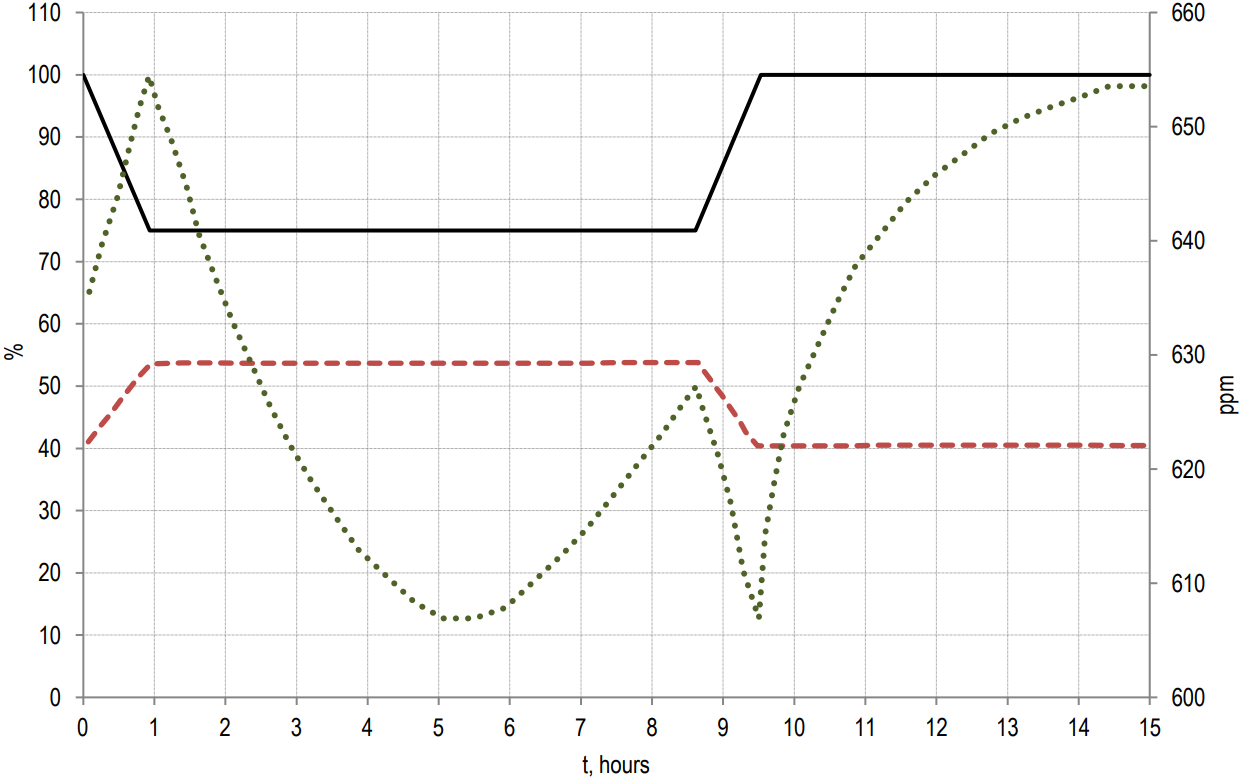
\includegraphics[width=0.7\textwidth]{content/figures/seguimiento_carga_barras_y_boro.png}
  \caption{Ejemplo de variación de potencia mediante la inserción del banco de barras de control D y la variación de la concentración de ácido bórico en un reactor \acrshort{pwr} (\cite{NEA_2011_load_following}).}
  \label{fig:seguimiento_carga_barras_y_boro}
\end{figure}

Tal y como se ha comentado al inicio de este subapartado, es preferible mantener el reactor operando constantemente a su máxima potencia, evitando así el ciclado térmico de los componentes del núcleo del reactor y del circuito primario. Por eso, los diseños de \acrshort{smr} más recientes apuestan principalmente por mantener siempre el circuito primario de la planta a plena potencia y seguir la curva de carga utilizando la energía ---tanto térmica como eléctrica--- del lado secundario para la cogeneración Una opción muy atractiva es la \textbf{derivación de vapor/turbina}. Cuando la demanda de electricidad en la red eléctrica cambia, el operador de la central puede ajustar la cantidad de vapor que pasa a través de la turbina principal utilizando válvulas de derivación. Al abrirlas, parte del vapor se desvía y no pasa por la turbina, lo que reduce la cantidad de energía que se convierte en electricidad (\cite{ANS_2019}). Este vapor puede emplearse para disintos fines, como calefacción urbana, desalación, producción de hidrógeno, etc. tal y como se detalla en el apartado de \textit{Cogeneración (\ref{cogeneracion})}. 

\subsubsection{Efectos del xenón ante variaciones de potencia}

Durante la operación de un reactor nuclear se acumula una gran cantidad de productos de fisión. Entre ellos, hay que prestar especial atención al $Xe^{135}$, cuya sección eficaz de captura neutrónica en el rango térmico es muy elevada, actuando como ``veneno del reactor'' e introduciendo reactividad negativa al mismo. El efecto de este envenenamiento ---que se pone especialmente de manifiesto en las operaciones de arranque, parada y variaciones de potencia--- debe tenerse muy en cuenta a la hora de diseñar y operar un reactor térmico.

El $Xe^{135}$ aparece directamente como un producto de fisión y por desintegración del $I^{135}$. A su vez, desaparece por captura y por decaimiento.

\begin{figure}[h]
  \centering
  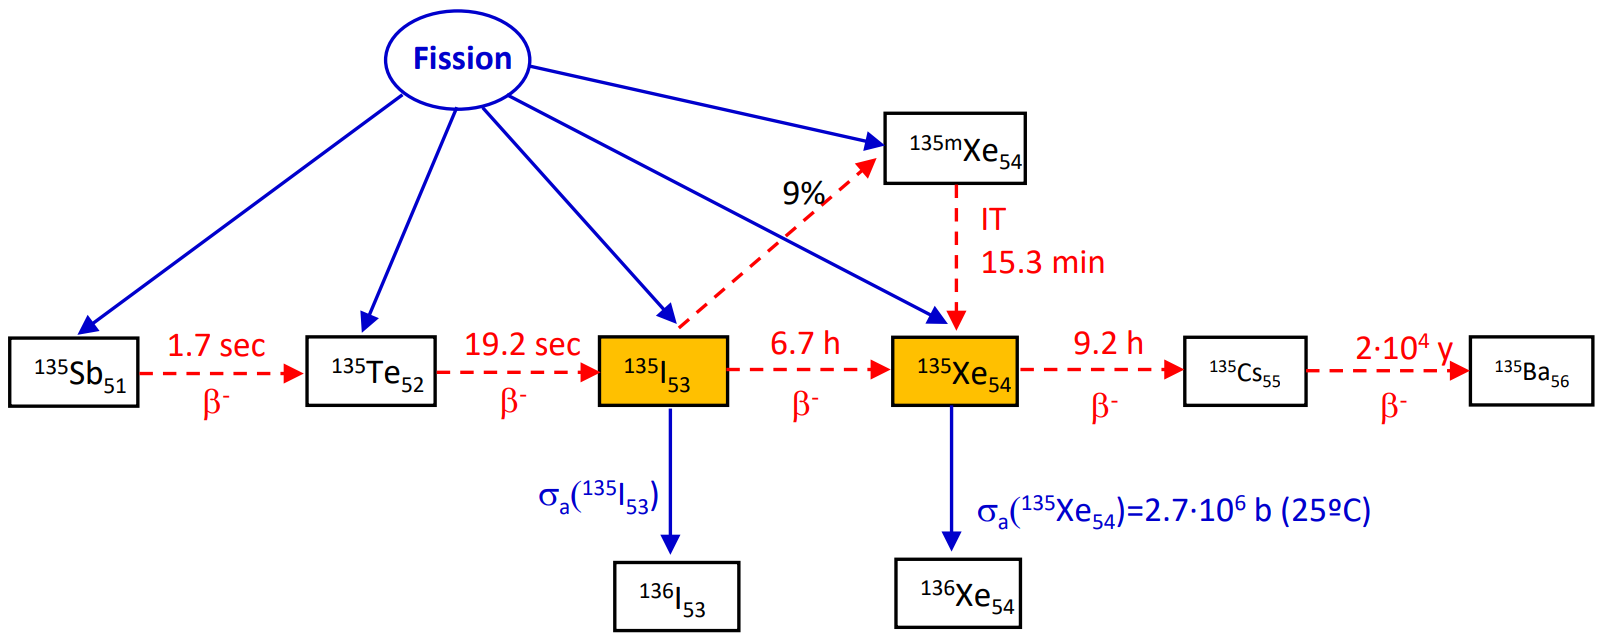
\includegraphics[width=0.8\textwidth]{content/figures/esquema_xenon.png}
  \caption{Esquema completo de aparición y desparación del $Xe^{135}$ (\cite{apuntes_centrales}).}
  \label{fig:esquema_xenon}
\end{figure}

Asumiendo que las desintegraciones del $Te^{135}$ y del $Sb^{135}$ son instantáneas ---y se combinan los rendimientos de fisión en los denominados \textit{rendimientos de fisión acumulados ($\gamma$)}---, que el decaimiento del $Cs^{135}$ es despreciable y que la absorción del $I^{135}$ es despreciable comparada con su decaimiento, se obtiene el esquema simplificado de aparición y desaparición del $Xe^{135}$ mostrado en la figura \ref{fig:esquema_xenon_simplificado}, con la siguiente evolución temporal:

\begin{figure}[h]
  \centering
  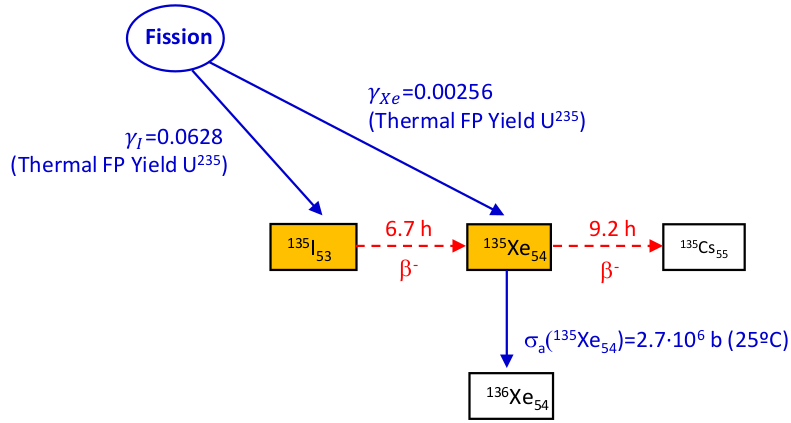
\includegraphics[width=0.7\textwidth]{content/figures/esquema_xenon_simplificado.png}
  \caption{Esquema simplificado de aparición y desparación del $Xe^{135}$ (\cite{apuntes_centrales}).}
  \label{fig:esquema_xenon_simplificado}
\end{figure}

\begin{equation} \label{evolucion_xenon}
  \frac{d X e}{d t}=\gamma_{X e} \cdot \Sigma_f \cdot \Phi+\lambda_I \cdot I-\left(\lambda_{X e}+\sigma_a^{X e} \cdot \Phi\right) \cdot X e
\end{equation}

En lo que respecta al seguimiento de carga, interesa conocer la evolución del xenón tras los cambios de potencia. 

En primer lugar, hay que tener en cuneta que el principal término fuente del $Xe^{135}$ es el decaimiento del $I^{135}$ y que el principal término sumidero es la captura. Analizando la ecuación \ref{evolucion_xenon} puede observarse que una disminución del flujo neutrónico ($\upsilon$) ---en el caso de una disiminución de potencia del reactor--- implica la reducción del término sumidero de  $Xe^{135}$, lo que conlleva un incremento en la cantidad del mismo no indefinido, ya que pasado un tiempo el xenón alcanza un nuevo estado de equilibrio. Por otro lado, un aumento en el flujo neutrónico ---en el caso de un aumento dee la potencia del reactor--- conlleva una consecuente disminución en la cantidad de $Xe^{135}$. Estas fluctuaciones en la cantidad de xenón inducen transitorios de reactividad que
originan oscilaciones espacio-temporales del flujo neutrónico en reactores con flujos elevados.

\begin{figure}[h]
  \centering
  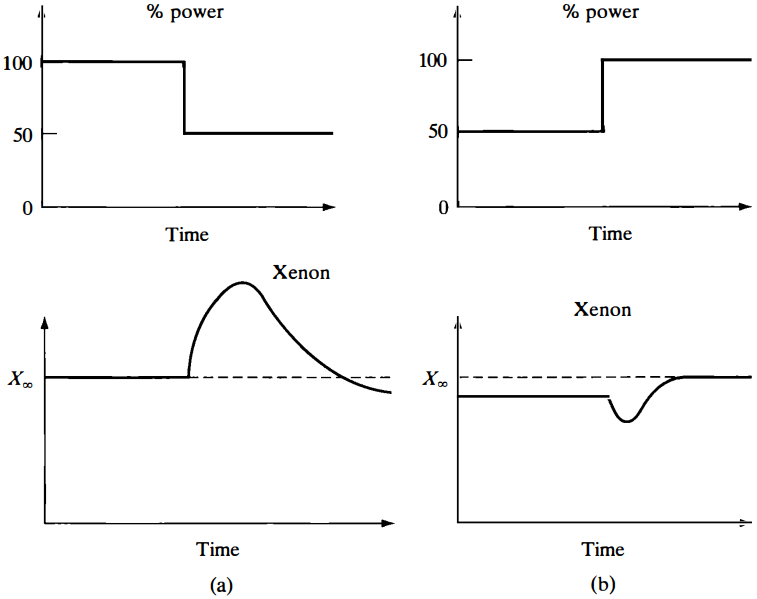
\includegraphics[width=0.65\textwidth]{content/figures/variaciones_potencia_xenon.png}
  \caption{Variaciones de la cantidad de $Xe^{135}$ al producirse variaciones en el flujo neutrónico (\cite{apuntes_centrales}).}
  \label{fig:variaciones_potencia_xenon}
\end{figure}

\subsection{Simulación de una maniobra completa de seguimiento de carga}

\subsection{Elaboración de una práctica para los alumnos del máster}